%%%%%%%%%%%%%%%%%%%%%%%%%%%%%%%%%%%%%%%%%
% University/School Laboratory Report
% LaTeX Template
% Version 3.1 (25/3/14)
%
% This template has been downloaded from:
% http://www.LaTeXTemplates.com
%
% Original author:
% Linux and Unix Users Group at Virginia Tech Wiki 
% (https://vtluug.org/wiki/Example_LaTeX_chem_lab_report)
%
% License:
% CC BY-NC-SA 3.0 (http://creativecommons.org/licenses/by-nc-sa/3.0/)
%
%%%%%%%%%%%%%%%%%%%%%%%%%%%%%%%%%%%%%%%%%

%----------------------------------------------------------------------------------------
%	PACKAGES AND DOCUMENT CONFIGURATIONS
%----------------------------------------------------------------------------------------

\documentclass{article}

\usepackage[version=3]{mhchem} % Package for chemical equation typesetting
\usepackage{siunitx} % Provides the \SI{}{} and \si{} command for typesetting SI units
\usepackage{graphicx} % Required for the inclusion of images
\usepackage{natbib} % Required to change bibliography style to APA
\usepackage{amsmath} % Required for some math elements 
\usepackage{listings}
\usepackage{xcolor}


\definecolor{codegreen}{rgb}{0,0.6,0}
\definecolor{codegray}{rgb}{0.5,0.5,0.5}
\definecolor{codepurple}{rgb}{0.58,0,0.82}
\definecolor{backcolour}{rgb}{0.95,0.95,0.92}

\lstdefinestyle{mystyle}{
    backgroundcolor=\color{backcolour},   
    commentstyle=\color{codegreen},
    keywordstyle=\color{magenta},
    numberstyle=\tiny\color{codegray},
    stringstyle=\color{codepurple},
    basicstyle=\ttfamily\footnotesize,
    breakatwhitespace=false,         
    breaklines=true,                 
    captionpos=b,                    
    keepspaces=true,                 
    numbers=left,                    
    numbersep=5pt,                  
    showspaces=false,                
    showstringspaces=false,
    showtabs=false,                  
    tabsize=2
}

\lstset{style=mystyle}

\setlength\parindent{0pt} % Removes all indentation from paragraphs

\renewcommand{\labelenumi}{\alph{enumi}.} % Make numbering in the enumerate environment by letter rather than number (e.g. section 6)

%\usepackage{times} % Uncomment to use the Times New Roman font

%----------------------------------------------------------------------------------------
%	DOCUMENT INFORMATION
%----------------------------------------------------------------------------------------

\title{REMODEL- A Community Poll on Reproducibility in Computational Geosciences} % Title

\author{Robert \textsc{Reinecke}} % Author name

\date{\today} % Date for the report

\begin{document}

\maketitle % Insert the title, author and date

\begin{center}
\begin{tabular}{l r}
Report last updated: & 17th May, 2021 \\ % Date
\end{tabular}
\end{center}

This document summerizes a full analysis for detailed results. \textbf{It is not a full publication but rather an automated representation of the data present in this repository}

It summarizes the extensive results and builds the foundation for the publication of a journal paper.
It will also be distributed along with the data in the course of a journal and data publication.

\section{Aim of this survey}
Software development has become an integral part of the geosciences¹ as models and data processing get more sophisticated. Paradoxically, it poses a threat to scientific progress as the pillar of science, reproducibility, is seldomly reached². Software code tends to be either poorly written and documented or not shared at all; proper software licenses are rarely attributed. This is especially worrisome as scientific results have potential controversial implications for stakeholders and policymakers and may influence the public opinion for a long time³.

In recent years, progress towards open science has led to more publishers demanding access to data and source code alongside peer-reviewed manuscripts4,5. Still, recent studies find that results can rarely be reproduced6,7.

In this project, we conduct a poll among the geoscience community which is advertised via scientific blogs (AGU, EGU), research networks (researchgate.net and mailing lists), and social media. Therein, we strive to investigate the causes for that lack of reproducibility. We take a peek behind the curtain and unveil how the community develops and maintains complex code and what that entails for reproducibility8. Our survey includes background knowledge, community opinion, and behaviour practices regarding reproducible software development.

We postulate that this lack of reproducibility9 might be rooted in insufficient reward within the scientific community, insecurity regarding proper licencing of software and other parts of the research compendium as well as scientists’ unawareness about how to make software available in a way that allows for proper attribution of their work. We question putative causes such as unclear guidelines of research institutions or that software has been developed over decades10, by researchers' cohorts without a proper software engineering process¹ and transparent licensing.

To this end, we also summarize solutions like the adaption of modern project management methods from the computer engineering community11 that will eventually reduce costs while increasing the reproducibility of scientific research8.

1 A comment to "Most Computational Hydrology is not Reproducible, so is it Really Science?” R.W. Hut, N.C. van de Giesen, N. Drost, Water Resources Research, 2017

2 Hutton, C., Wagener, T., Freer, J., Han, D., Du\_y, C., and Arheimer, B., Most computational hydrology is not reproducible, so is it really science? Water Resources Research, 2016

3 Munafò, M., Nosek, B., Bishop, D. et al., A manifesto for reproducible science. Nat Hum Behav, 2017

4 Executive editors, G. Editorial: The publication of geoscientifc model developments v1.2. Geoscientifc Model Development, 2019

5 Katz, D. S., Niemeyer, K. E., and Smith, A. M., Publish your software: Introducing the journal of open source software (joss), Computing in Science Engineering, 2018

6 Stagge, J. H., Rosenberg, D. E., Abdallah, A. M., Akbar, H., Attallah, N. A., and James, R., Assessing data availability and research reproducibility in hydrology and water resources. Scientific data, 2019

7 Añel, J. A., García-Rodríguez, M., and Rodeiro, J.: Current status on the need for improved accessibility to climate models code, Geosci. Model Dev., 2021.

8 Stodden, V., The reproducible research standard: Reducing legal barriers to scientific knowledge and innovation. IEEE Computing in Science \& Engineering, 2009

9 https://www.nature.com/news/1-500-scientists-lift-the-lid-on-reproducibility-1.19970

10 Muller, C., Schaphoff, S., von Bloh, W., Thonicke, K., and Gerten, D., Going open-source with a model dinosaur and establishing model evaluation standards. EGU, 2018

11 https://software.rajivprab.com/2019/11/25/the-birth-of-legacy-software-how-change-aversion-feeds-on-itself
Our larger questions:
\begin{itemize}
	\item Is eproducibility is an issue in the geosciences? Are bad code and documentation the root cause of that issue?
	\item Is model software too complex? Does that hinder reproducibility?
	\item Are researchers missing the tools and know-how (methods, licenses etc.) to build good model code?
	\item Is missing funding and missing time preventing researchers from making their models more accessible?
\end{itemize}

We define reproducibility as:

"Reproducibility in the context of modeling in the geosciences means that results obtained by a modeling experiment should be achieved again with a high degree of agreement when the study is replicated with the same model design, inputs, and general methodology by different researchers.

We explicitly exclude the retracing of results by means of using a different modeling environment (including variations in model concept, algorithms, input data or methodology)."

\section{Data processing}
We designed the survey according to standards from psychology research. We apply descriptive statistics to analyse demographic background and basic analysis.
Further, we apply inferential statistical methods to test the unerlying hypotheses.

The raw data of the survey is stored in the folder \textbf{LiveData}. \textbf{The raw data has not been modified or cleaned in any way.}
To run some basic cleanup run the follwoing script: 

\begin{lstlisting}[language=Python]
import process_data.py as p
p.process()
\end{lstlisting}

\section{Results}
All data processing and plotting (including building this document) can be executed by running \lstinline{python run.py}.
Plotting details and addtional processing can be found in th script \lstinline{plot_all.py}.

\subsection{Sample Characteristics (demographics)}
Who were our participants?
Here we present characteristics of the participants in our poll, i.e. their current career stage, their years of research experience, their geo-scientific field and scale as well as their current focus of work.
This is purely descriptive statistics.
As we welcomed everyone to our poll, we did not form any assumptions regarding sample characteristics.
Also, we tried, but might not have reached a representative sample of the population of geo-scientists.

Here, we report basic sample characteristics. Also, we can check for and report any salient sample properties.

Corresponding survey questions:

\begin{itemize}
	\item DM01 - What career stage are you in?
	\item DM02 - For how long have you been working in your research field?
	\item DM06 - To which field within the geosciences does your research mainly belong?
	\item DM05 - What geographic scale are you working on?
	\item DM07 - What is the focus of your work?
\end{itemize}

\begin{figure}[h!]
    \centering
    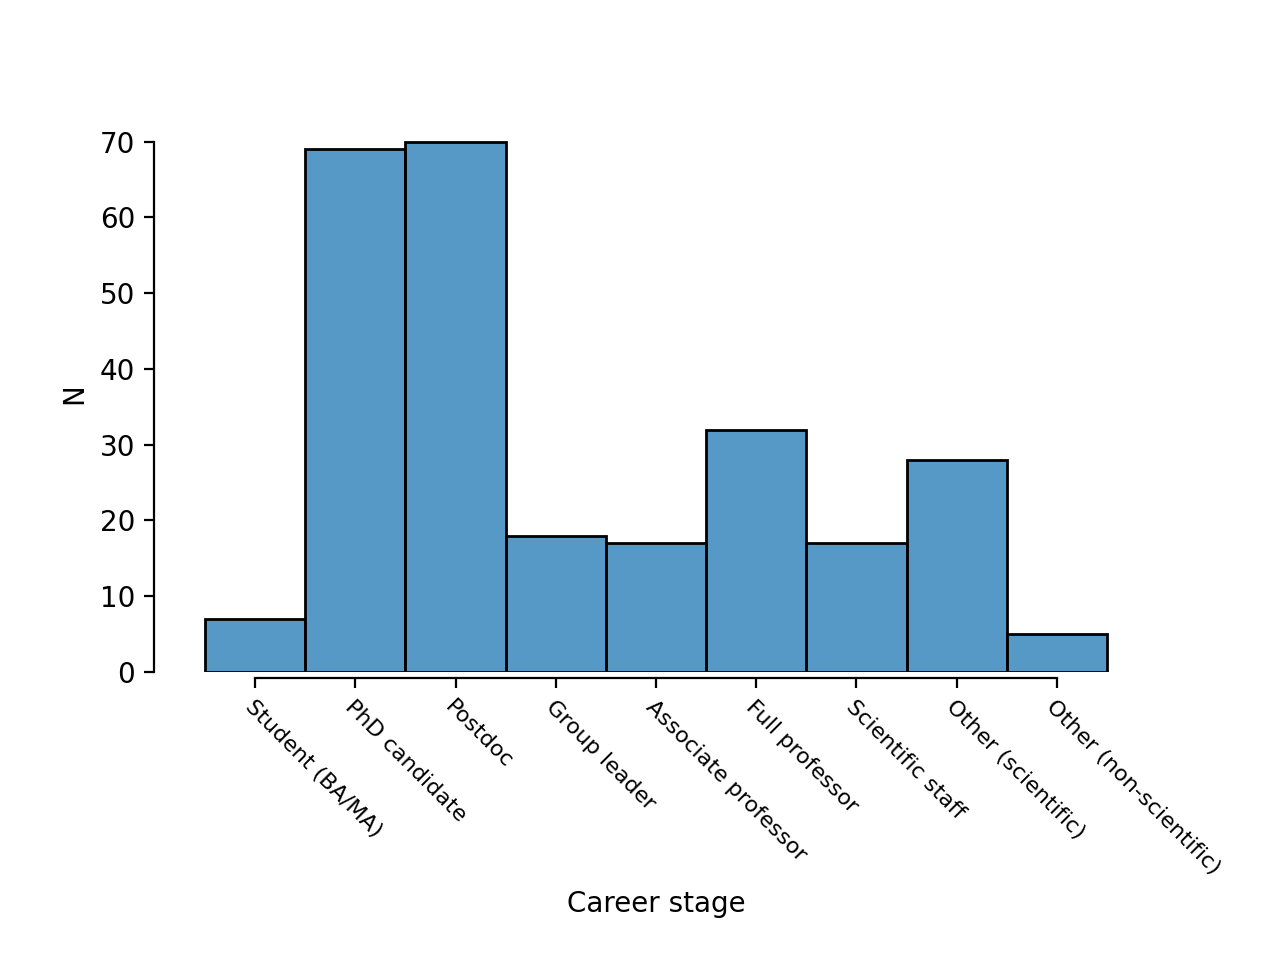
\includegraphics[width=\textwidth]{../figs/DM01.png}
	\caption{DM01 - Career stage of participants}
    \label{fig:dm01}
\end{figure}

\begin{figure}[h!]
    \centering
    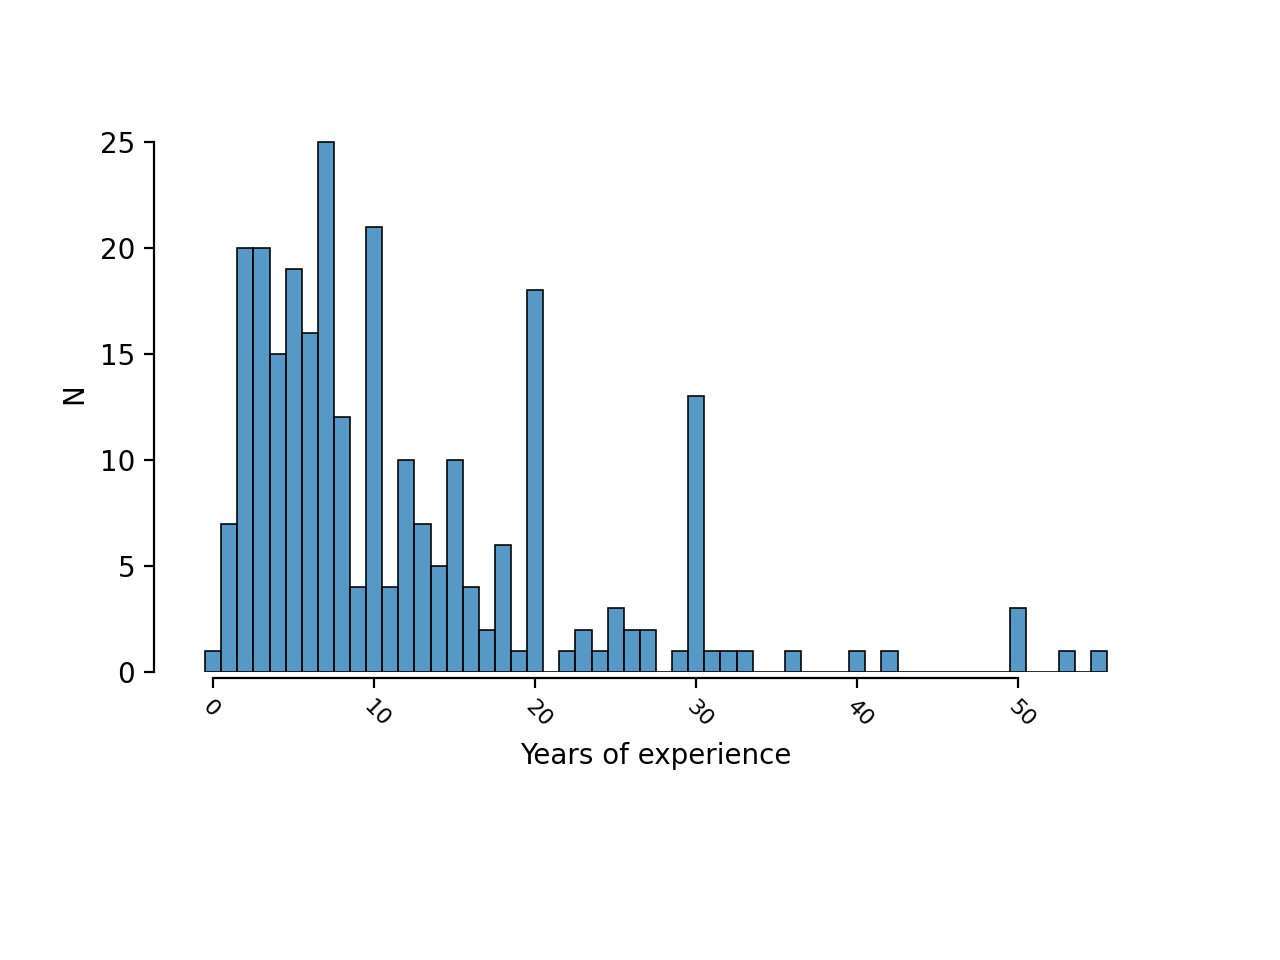
\includegraphics[width=\textwidth]{../figs/DM02_01.png}
	\caption{DM02 - For how long have you been working in your field?}
    \label{fig:dm02}
\end{figure}

\begin{figure}[h!]
    \centering
    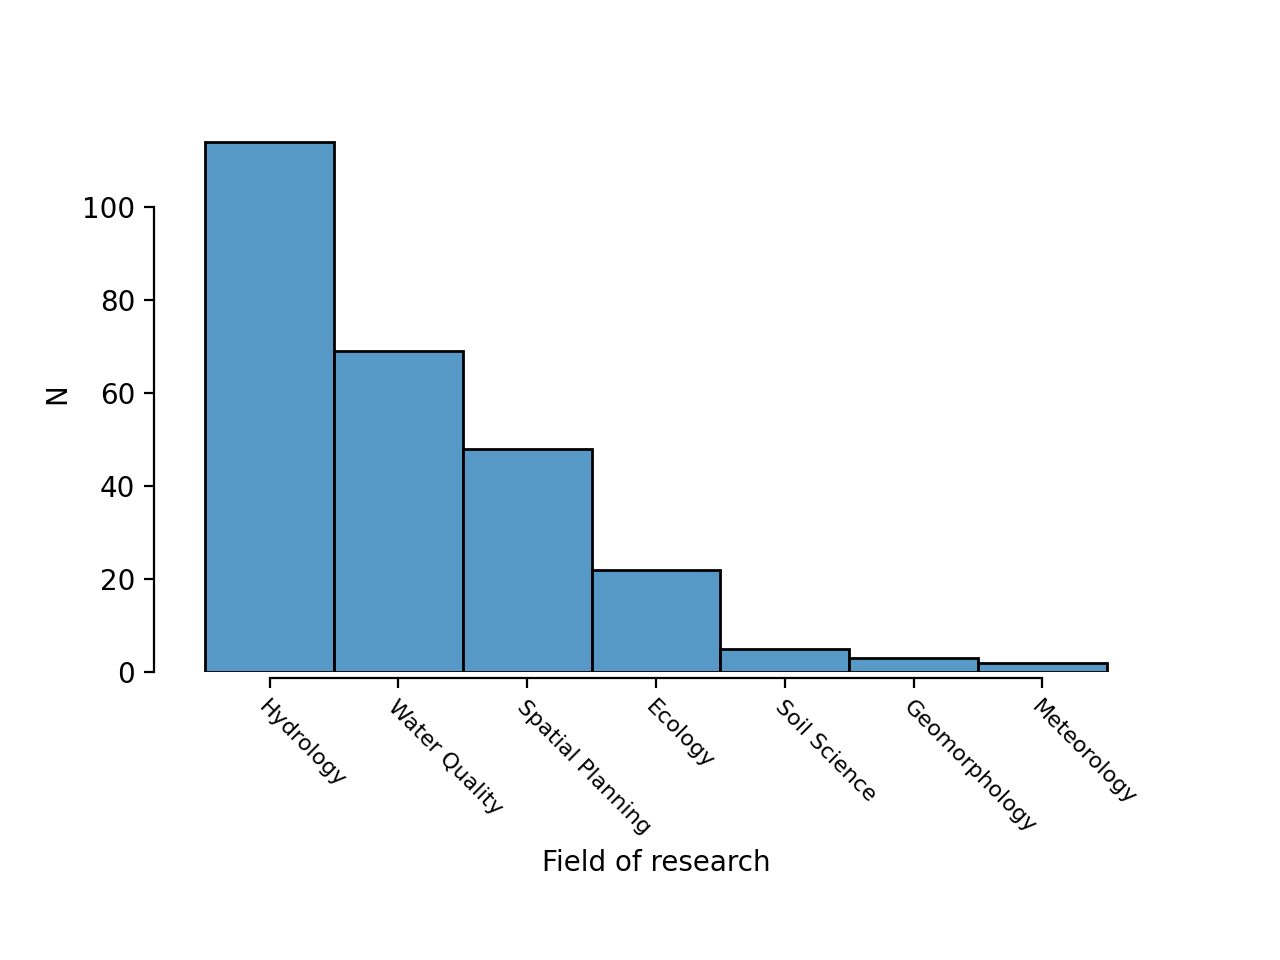
\includegraphics[width=\textwidth]{../figs/DM06.png}
	\caption{DM06 - Which field do you belong to?}
    \label{fig:dm06}
\end{figure}

\begin{figure}[h!]
    \centering
    \includegraphics[width=\textwidth]{../figs/DM05.png}
	\caption{DM05 - What scale are you working on?}
    \label{fig:dm05}
\end{figure}

\begin{figure}[h!]
    \centering
    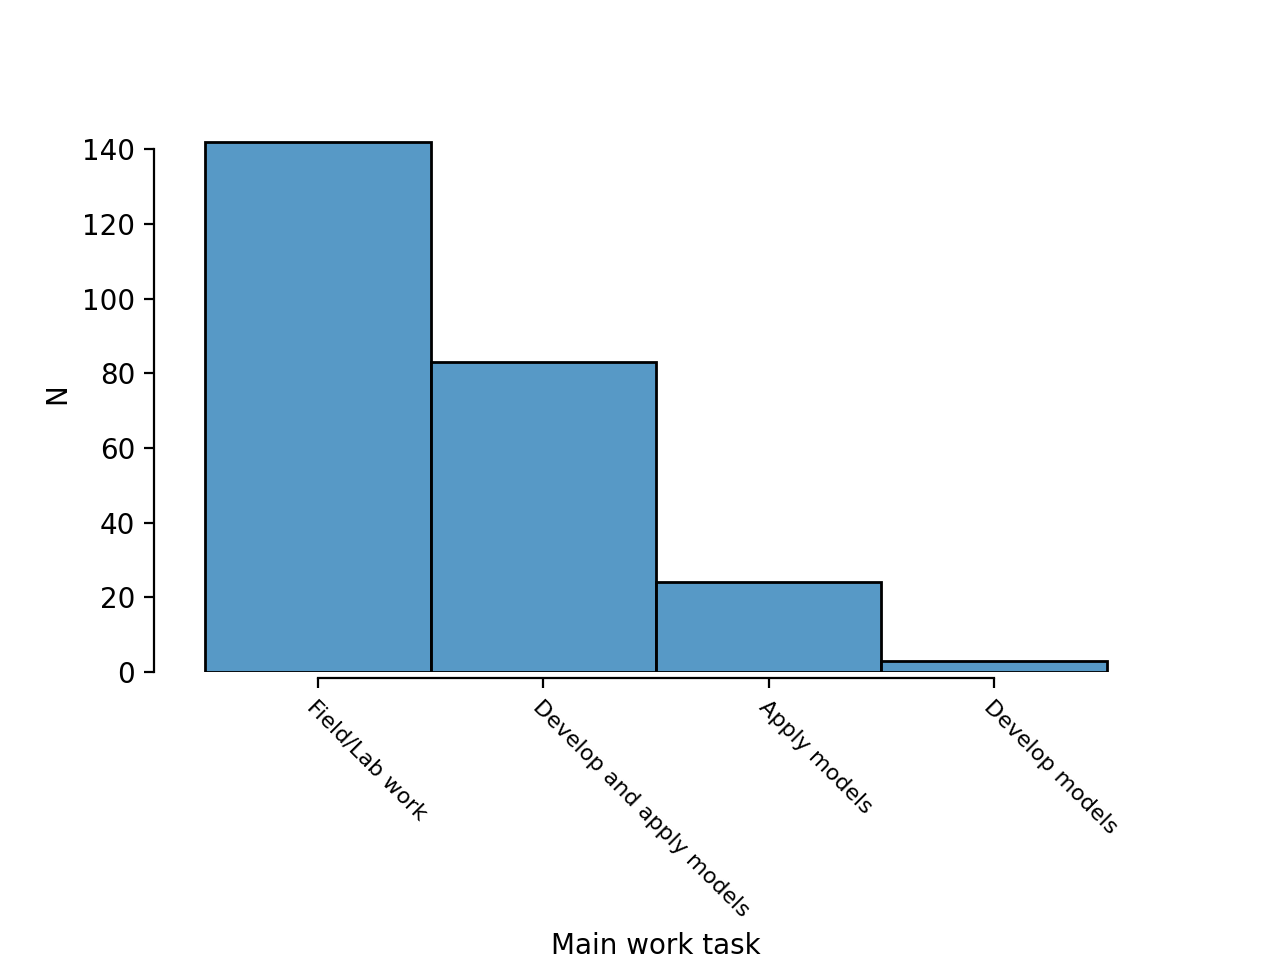
\includegraphics[width=\textwidth]{../figs/DM07.png}
	\caption{DM07 What is the focus of your work?}
    \label{fig:dm07}
\end{figure}

\subsection{Community Opinion on Reproducibility}

This part covers people's view and opinion.

Start here with summary of our hypotheses We assume that... (formulate in a neutral tone) TODOOOOOOO

Analysis Steps:
\begin{itemize}
	\item plot corresponding questions (across full sample)
	\item perform statistical testing of our above stated hypotheses (across subgroups, e.g. early career vs senior researcher)
	\item perform further data exploration (NOT hypothesis testing) - this might inspire future research, e.g. correlation analysis
\end{itemize}

    corresponding hypotheses TODO copy here:
        H1
        H8
        H10
        H11


Corresponding survey questions:
\begin{itemize}
	\item O101
	\item O103
	\item S113
\end{itemize}

O101: Opinion on Reproducibility in Geo-Sciences: How strongly did participants generally agree with statements?
Do they consider it a problem at all? Do they think that their work is reproducible?

\begin{figure}[h!]
    \centering
    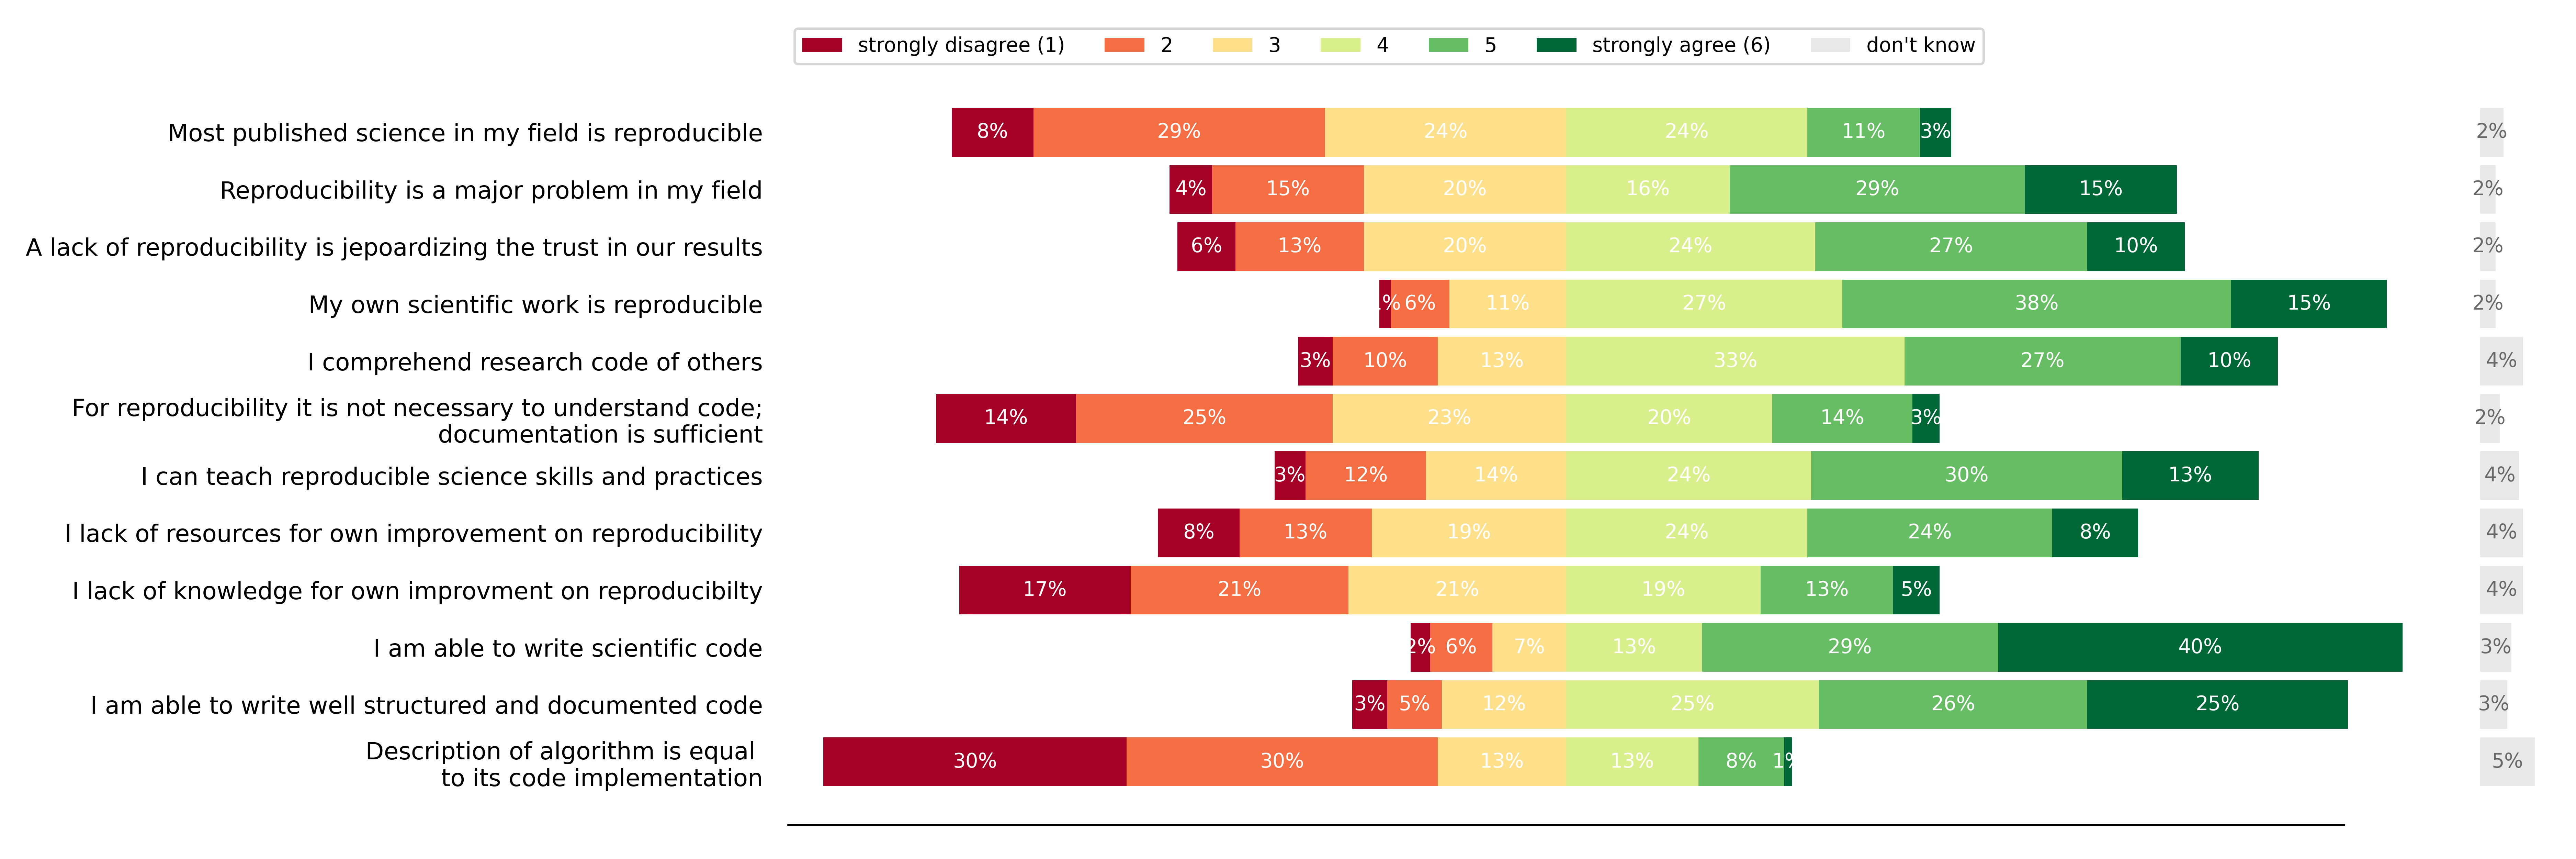
\includegraphics[width=\textwidth]{../figs/O101.png}
	\caption{O101 }
    \label{fig:O101}
\end{figure}



O101 (hypotheses): Differences in Opinion on Reproducibility in Geo-Sciences: Do early career researcher differ from senior researchers in their agreement?

 perform statistical test (chosen by scale and sample distribution)

 show test results

 show subgorup plot (according to hypotheses, e.g. early careers have )

O103: Reasons for lack of reproducibility: Rating of agreement to reasons

\begin{figure}[h!]
    \centering
    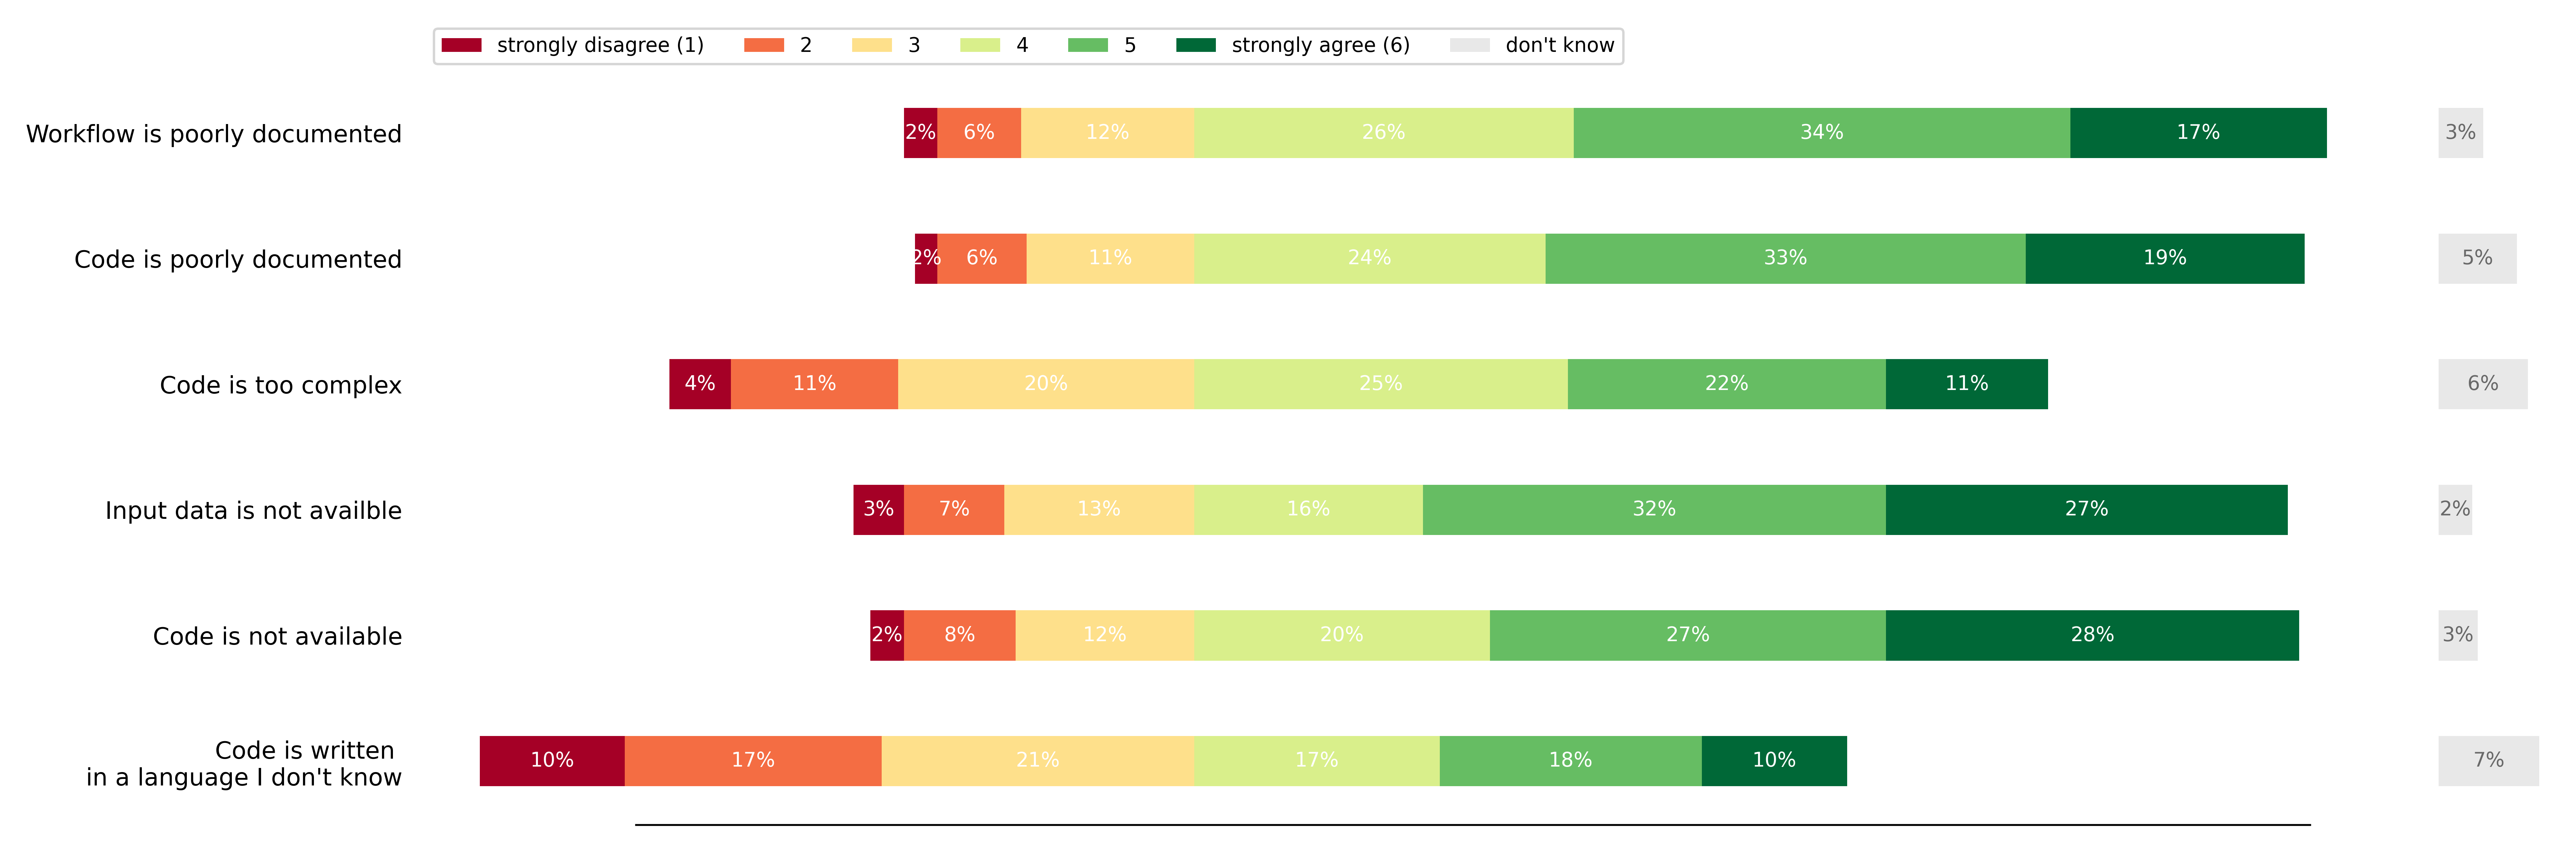
\includegraphics[width=\textwidth]{../figs/O103.png}
	\caption{O103 }
    \label{fig:O103}
\end{figure}

 perform hypothesis test

 explore data even further

 etc...

S113: Time for new students to get familiar with software

\begin{figure}[h!]
    \centering
    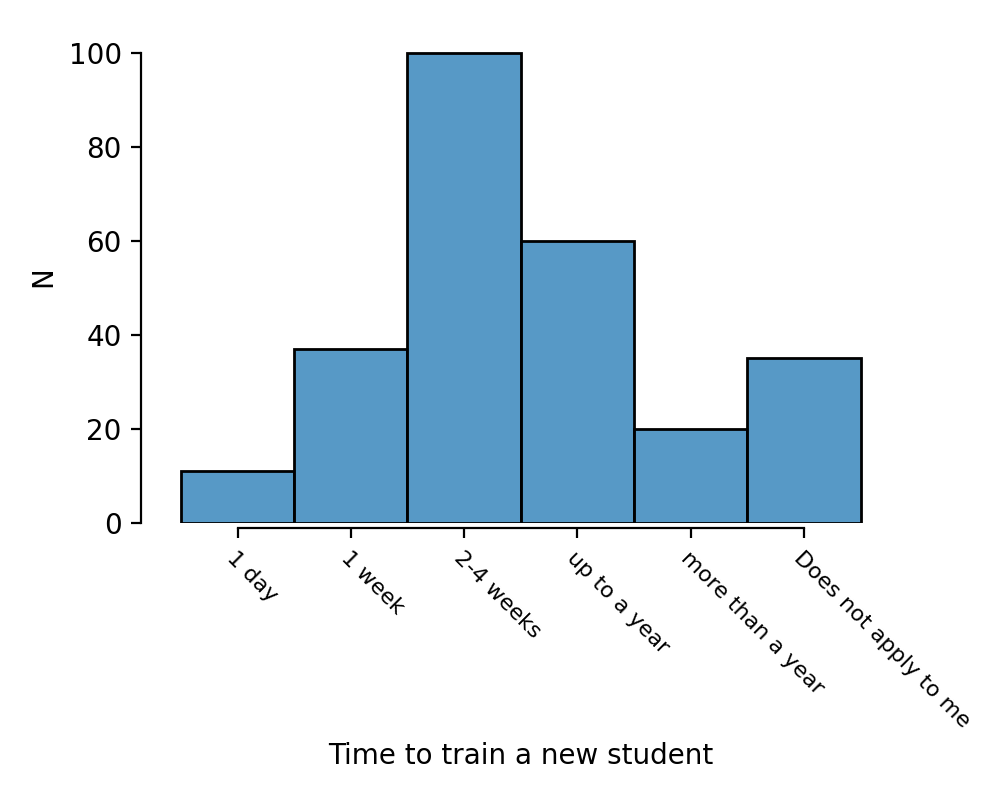
\includegraphics[width=\textwidth]{../figs/S113.png}
	\caption{S113 }
    \label{fig:S113}
\end{figure}


\subsection{Reproducibility Practices and Skills}

This part covers "actual" behaviour. (still only self-report assessment, but we can't change that)

    Start here with summary of our hypotheses

We expected to see that... (formulate in a neutral tone)

    Analysis Steps:
        plot corresponding questions (across full sample)
        perform statistical testing of our above stated hypotheses (across subgroups, e.g. early career vs senior researcher)
        perform further data exploration (NOT hypothesis testing) - this might inspire future research, e.g. correlation analysis

    corresponding hypotheses (see Robert's evaluation plan):
        H6
        H9
        H12
        H5
        H2

    Corresponding survey questions:
        O102
        S103
        S110
        S202
        S112
        S101
        S111
        S104
        S105
        S106

\begin{figure}[h!]
    \centering
    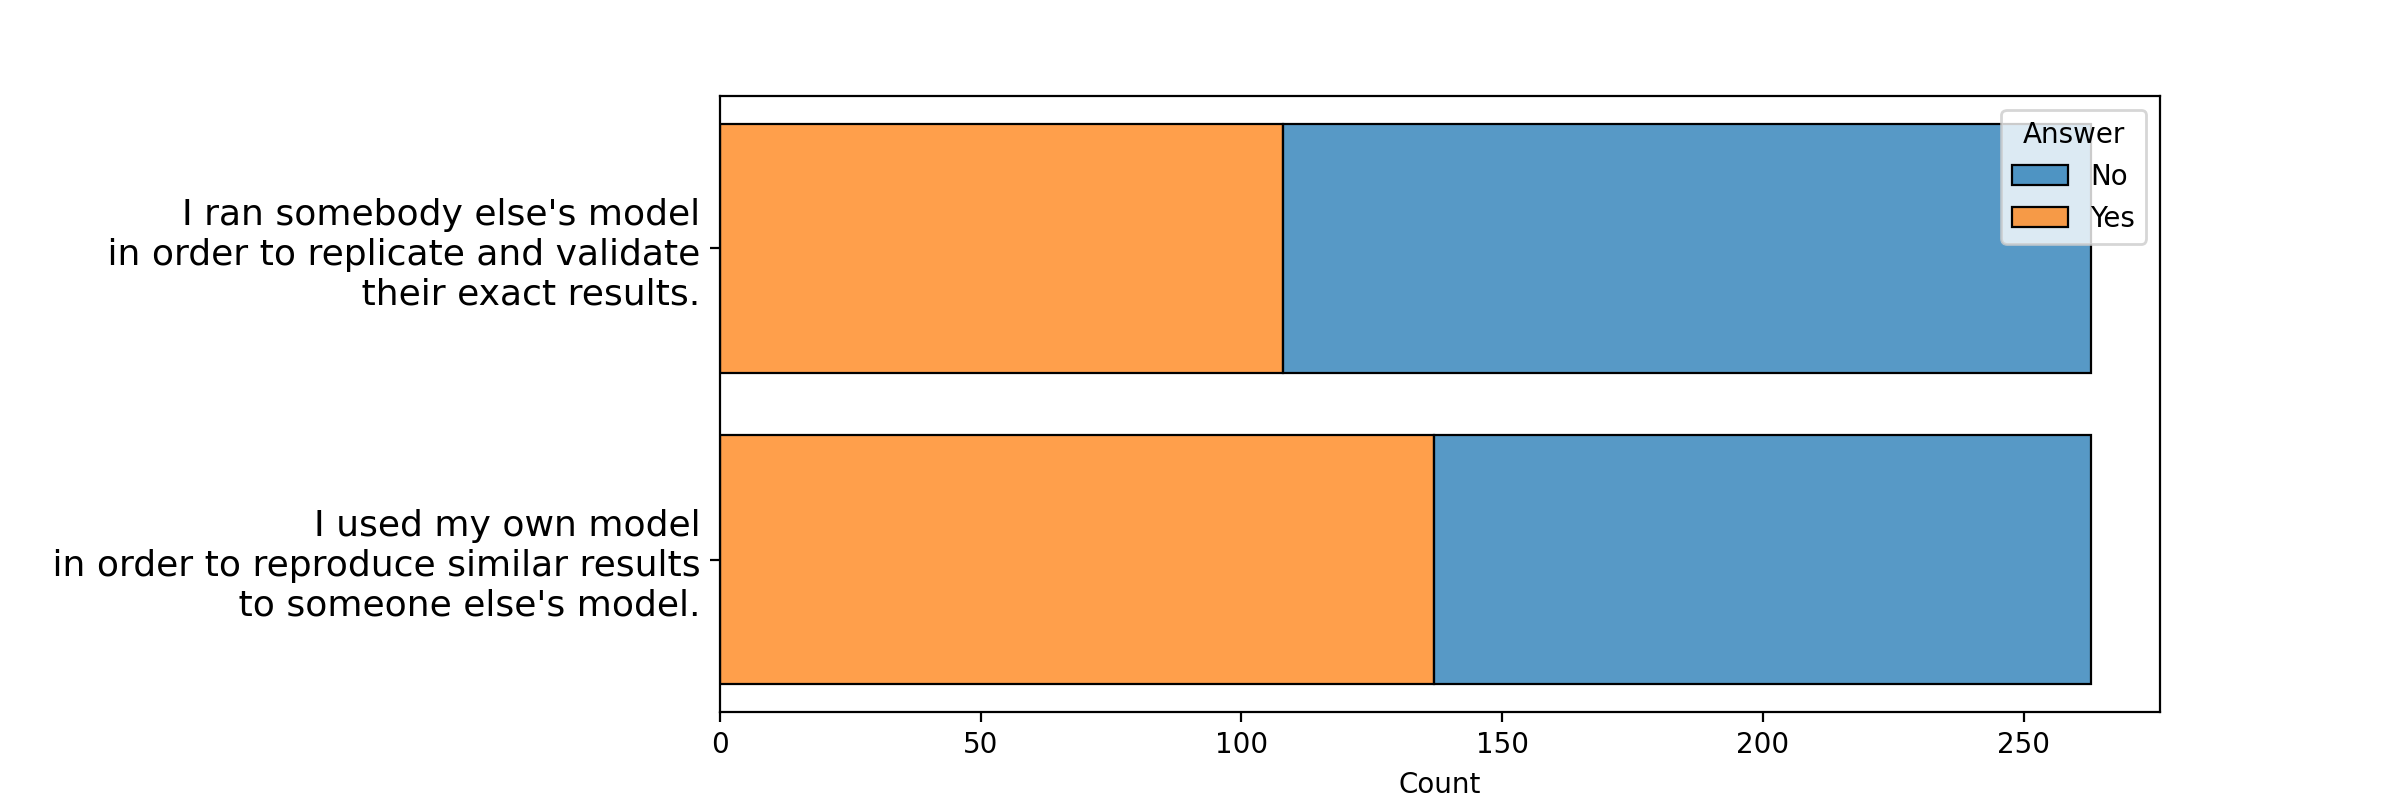
\includegraphics[width=\textwidth]{../figs/O102.png}
	\caption{O102 }
    \label{fig:O102}
\end{figure}

\begin{figure}[h!]
    \centering
    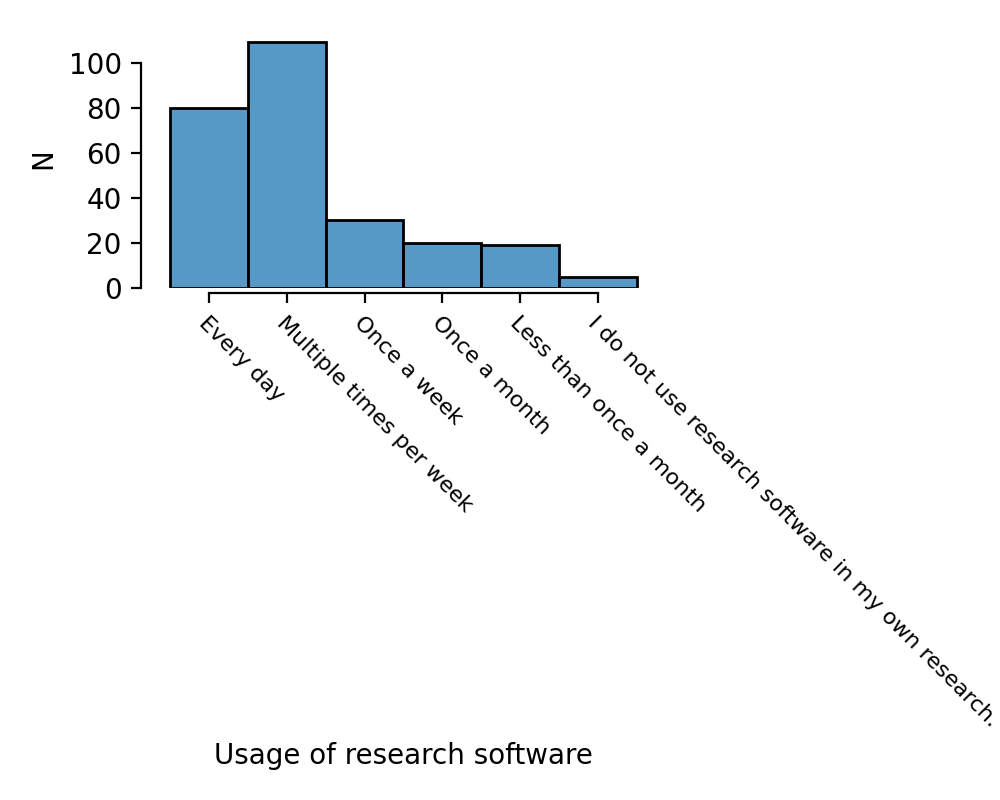
\includegraphics[width=\textwidth]{../figs/S103.png}
	\caption{S103 }
    \label{fig:S103}
\end{figure}

\begin{figure}[h!]
    \centering
    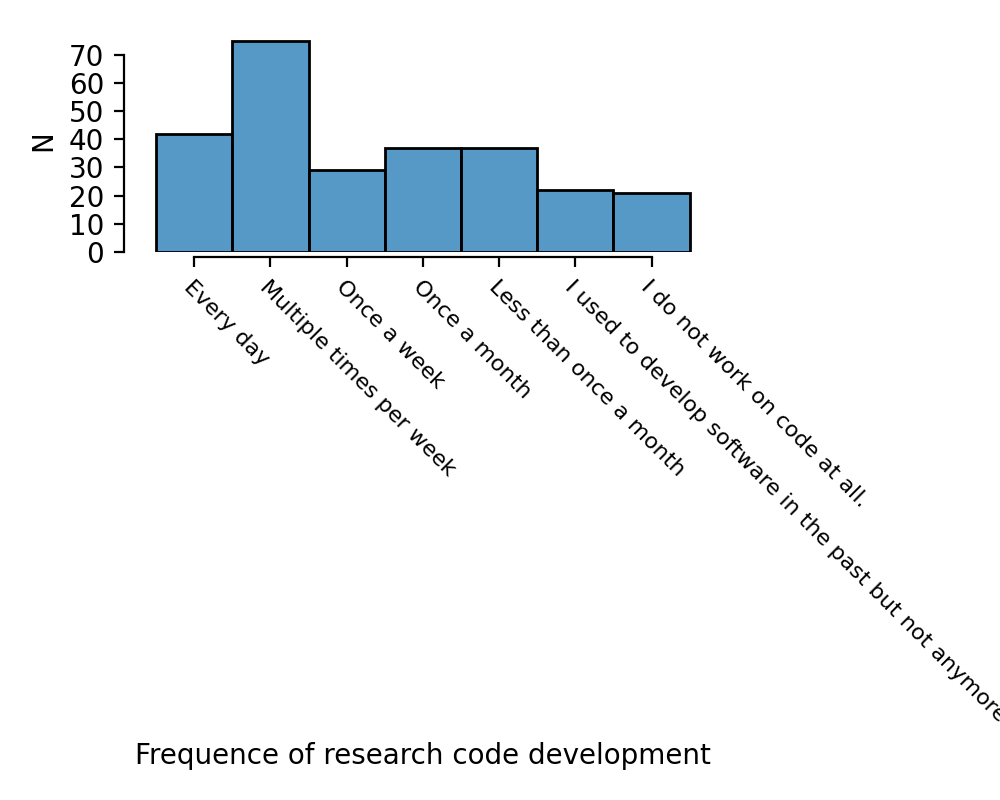
\includegraphics[width=\textwidth]{../figs/S110.png}
	\caption{S110 }
    \label{fig:S110}
\end{figure}

\begin{figure}[h!]
    \centering
    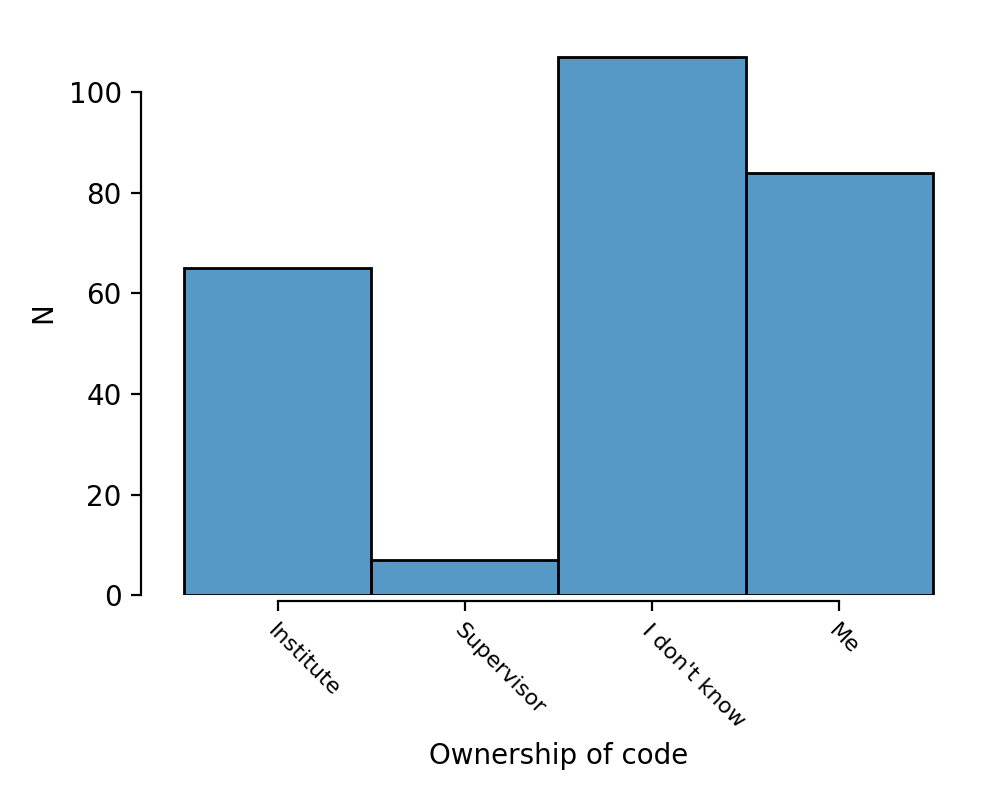
\includegraphics[width=\textwidth]{../figs/S202.png}
	\caption{S202 }
    \label{fig:S202}
\end{figure}

\subsection{Hurdles against and Solutions towards Reproducibility}

This part covers "actual" behaviour. (still only self-report assessment, but we can't change that)

    Start here with summary of our hypotheses

We stated that... (formulate in a neutral tone)

    Analysis Steps:
        plot corresponding questions (across full sample)
        perform statistical testing of our above stated hypotheses (across subgroups, e.g. early career vs senior researcher)
        perform further data exploration (NOT hypothesis testing) - this might inspire future research, e.g. correlation analysis

    corresponding hypotheses (see Robert's evaluation plan):
        H7
        H13
        H3

    Corresponding survey questions:
        S203
        S201
        S204 (open text)

\begin{figure}[h!]
    \centering
    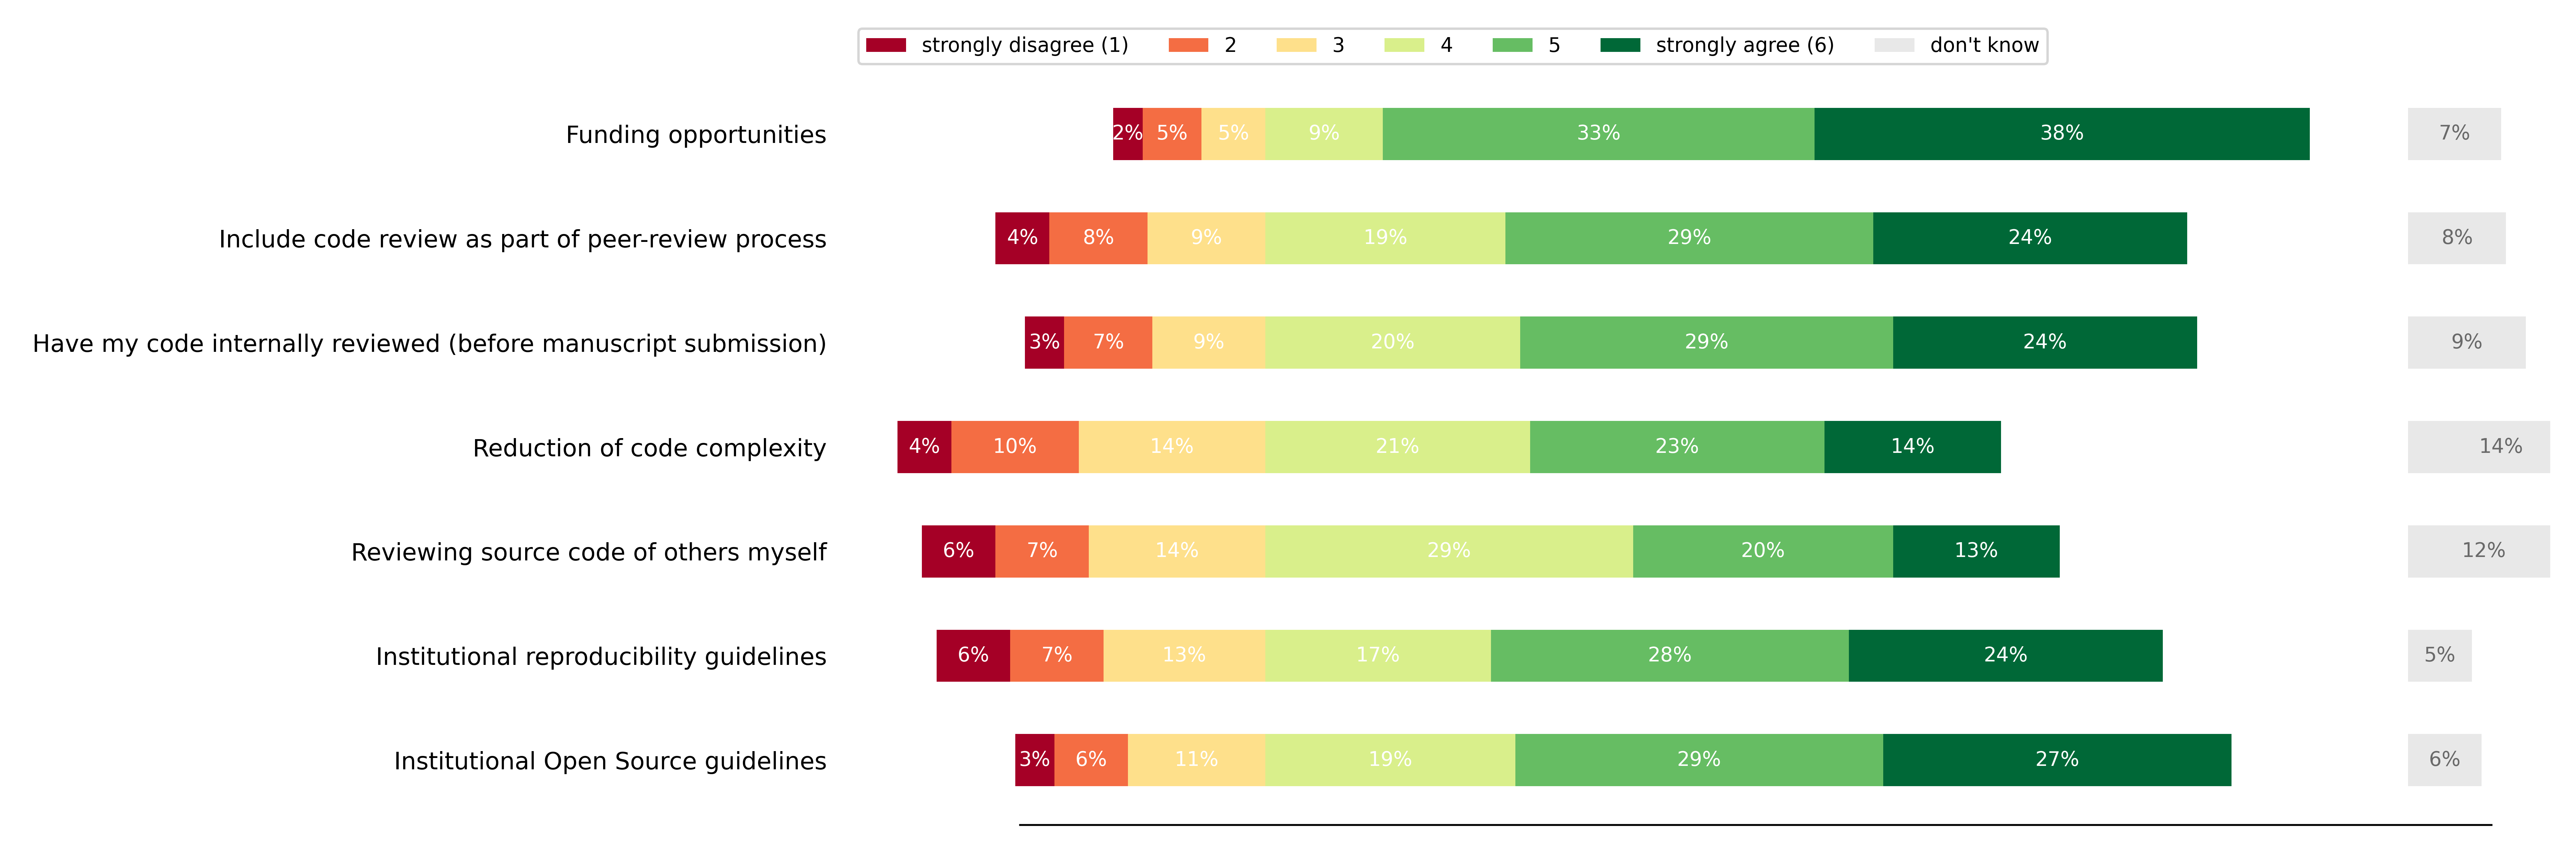
\includegraphics[width=\textwidth]{../figs/S201.png}
	\caption{S201 }
    \label{fig:S201}
\end{figure}

\begin{figure}[h!]
    \centering
    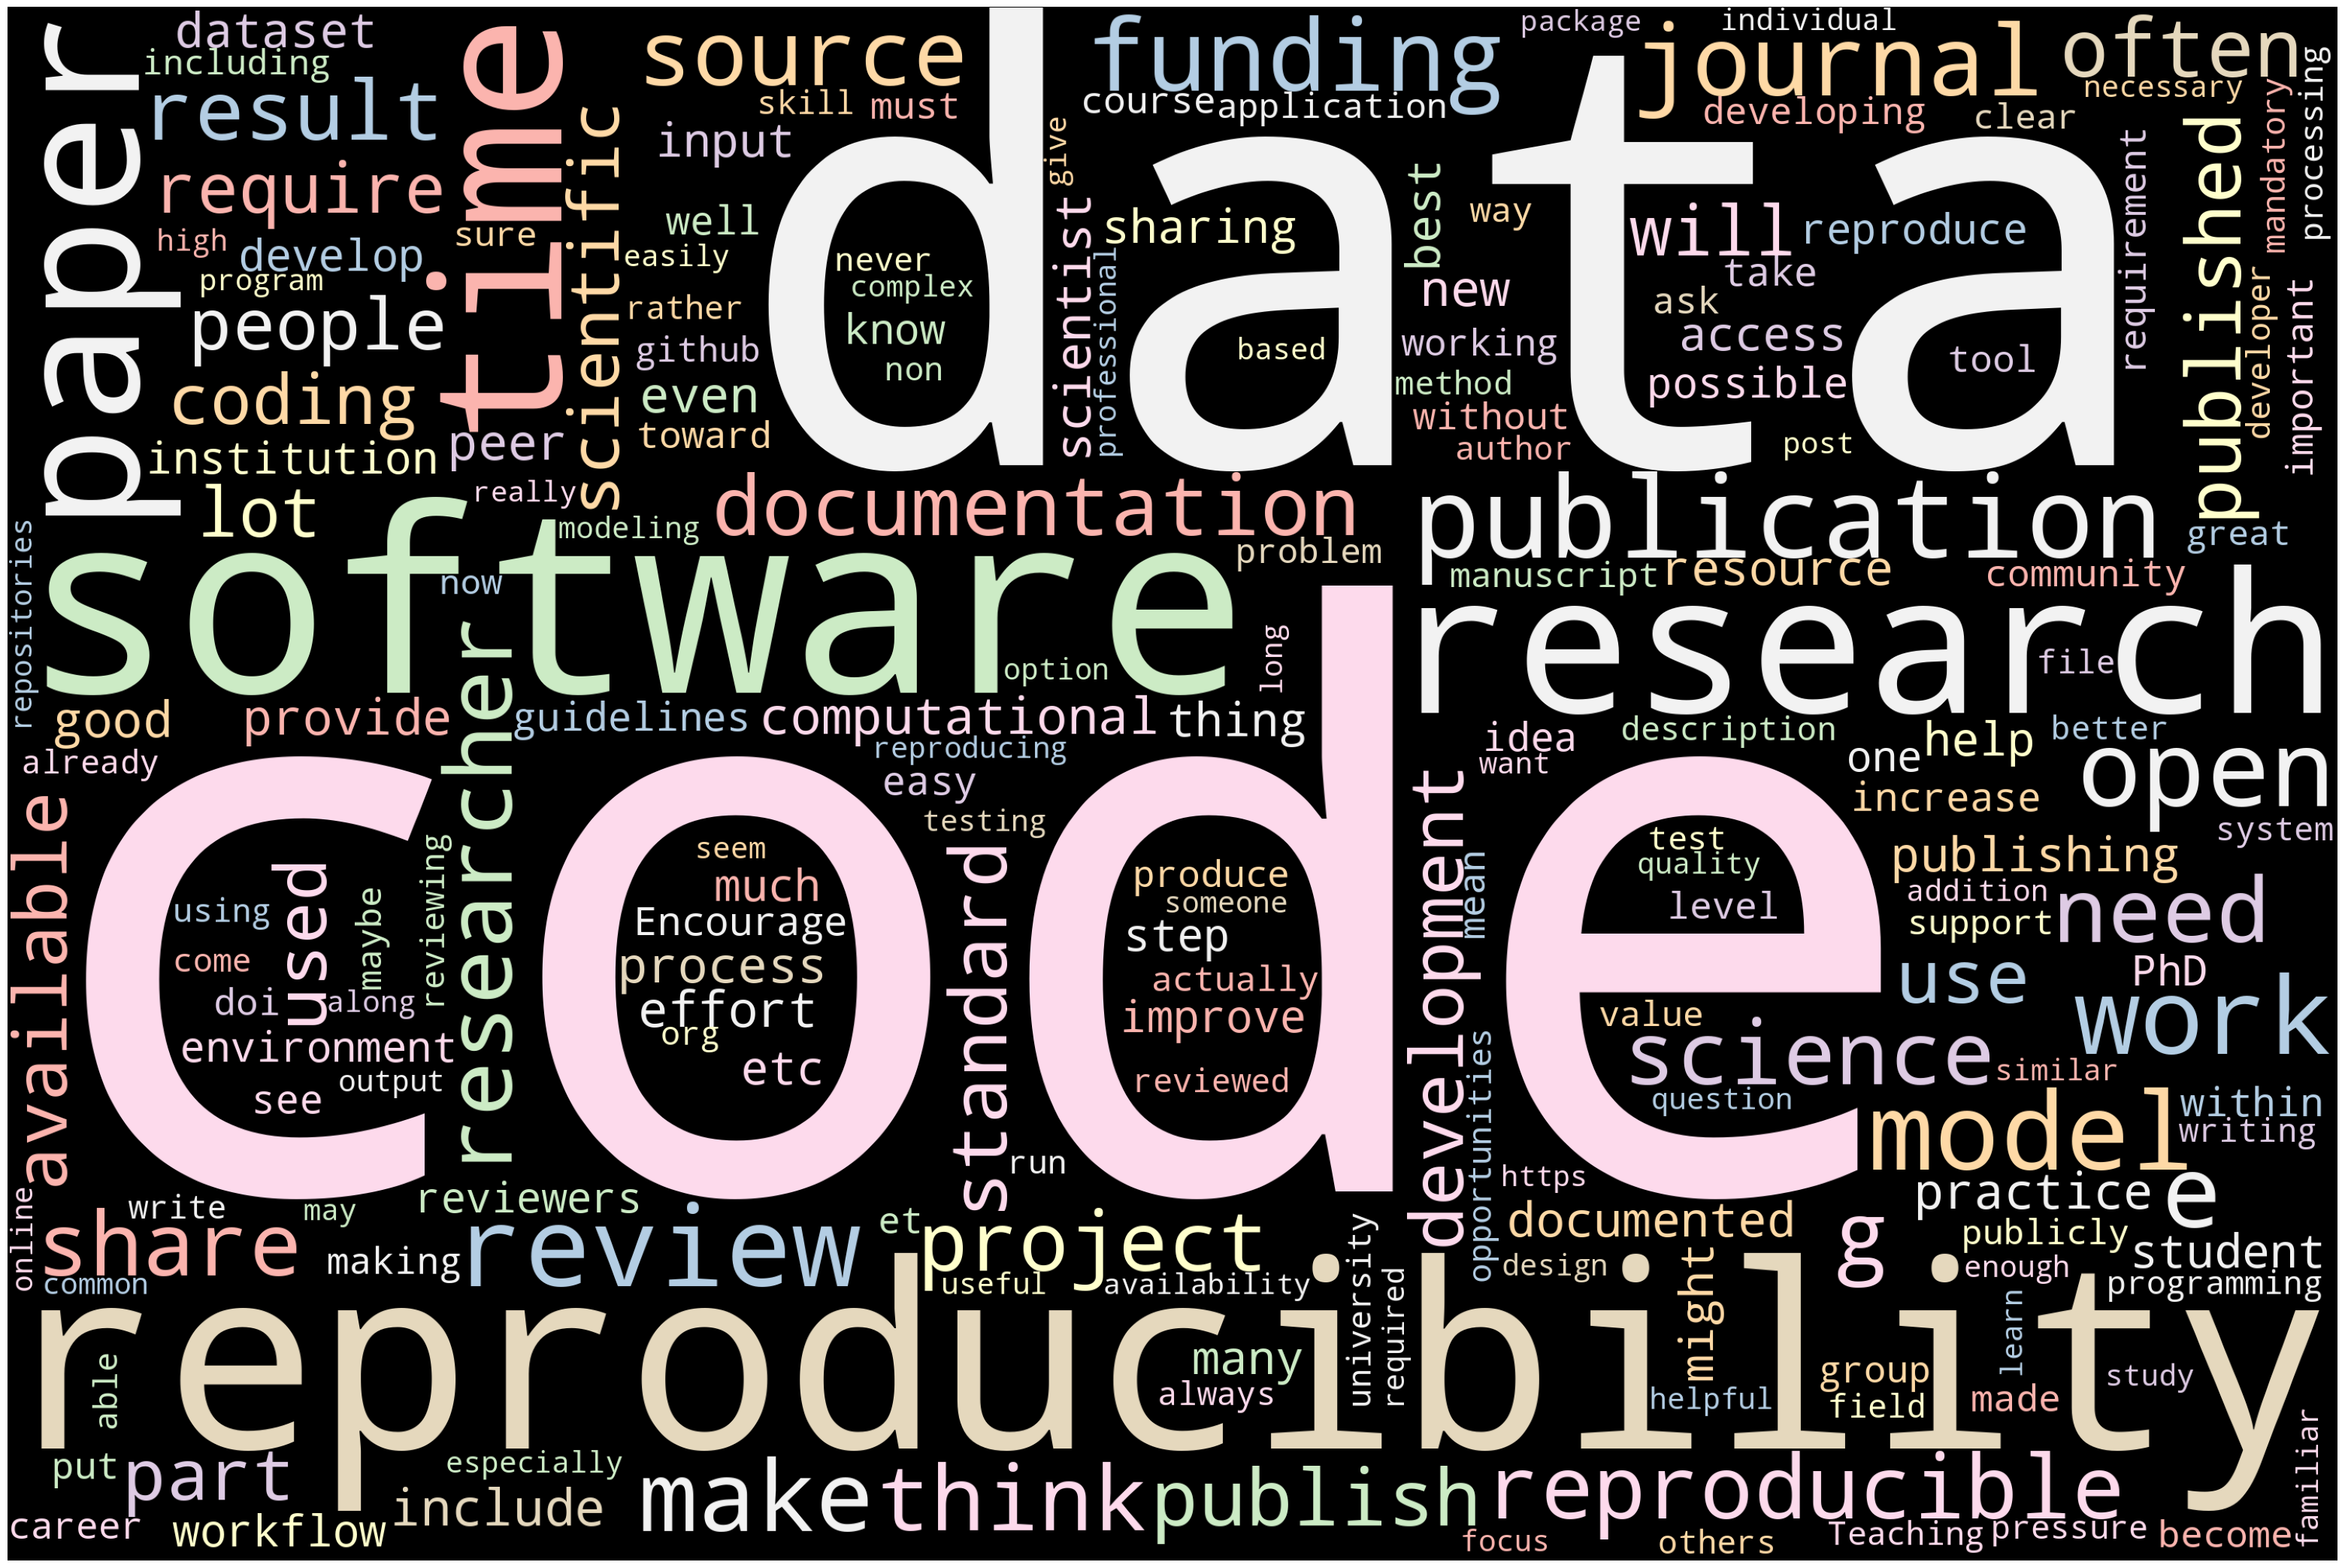
\includegraphics[width=\textwidth]{../word_cloud.png}
	\caption{Full text answers as word cloud }
    \label{fig:wc}
\end{figure}

\end{document}
